%% Template for COMP1204 coursework.

\documentclass[11pt,epsfig]{article}

\oddsidemargin=0in
\evensidemargin=0in
\textwidth=6.3in
\topmargin=-.5in
\textheight=9in

\parindent=0in
\pagestyle{empty}
\usepackage{verbatim}
\usepackage{amsmath}
\usepackage{graphicx}
\usepackage{appendix}

\begin{document}


% ooooooooooooooooooooooooooooooooooooooooooooooooooooooooooooooo
%                             COVER
% ooooooooooooooooooooooooooooooooooooooooooooooooooooooooooooooo 

\centerline{\Large \bf COMP1204: DB Coursework}        
\vfill 
   
Jonathan Keable \\                             %%%(Name) 
ID: 25616196\\				%%% ID
email: jek1g15@ecs.soton.ac.uk \\ %%% ECS username
10th April 2016 \hfill                             %%%(date of report)


\section{Relational Model and ERD}
The Relation R1 of the review can be defined as follows:

\begin{table}[!htbp]
\centering
\begin{tabular}{|l|l|}
\hline
\textbf{Attribute} & \textbf{Data Type} \\ \hline
\underline{ReviewID} & INTEGER \\ \hline
\underline{HotelID} & INTEGER \\ \hline
Hotel Average Overall & REAL \\ \hline
Hotel Average Price & INTEGER \\ \hline
Hotel URL & STRING \\ \hline
UserID & STRING \\ \hline
Content & STRING \\ \hline
Date & STRING \\ \hline
OverallRating & INTEGER \\ \hline
Value & INTEGER \\ \hline
Rooms & INTEGER \\ \hline
Location & INTEGER \\ \hline
Cleanliness & INTEGER \\ \hline
CheckIn/FrontDesk & INTEGER \\ \hline
Service & INTEGER \\ \hline
BusinessService & INTEGER \\ \hline
NoReaders Review & INTEGER \\ \hline
NoHelpful Review & INTEGER \\ \hline
\end{tabular}
\end{table}

Here the ReviewID and  HotelID are the primary key, with review IDs being unique within a hotels set of reviews.

The Main Functional Dependency of this relation would be:
\paragraph{}
\{ReviewID,HotelID\} $\rightarrow$ \{All other attributes\}
\paragraph{}
If a user can only post one review per Hotel then:
\paragraph{}
\{UserID, HotelID\} $\rightarrow$ \{All other attributes\} 
\paragraph{}
Or perhaps if a user can only post one review for a hotel each day then:
\paragraph{}
\{UserID, Date, HotelID\} $\rightarrow$ \{All other attributes\}
\paragraph{}
However because multiple reviews can be places as a guest under the name "Trip Advisor Member" these dependencies in fact do not work, so we have to use unique review IDs instead.
\paragraph{}
Also,
\paragraph{}
\{HotelID\} $\rightarrow$ \{Hotel Average Overall, Hotel Average Price, Hotel URL\}
\paragraph{}
In order to make the relation BCNF we should move these attributes into another relation:

\begin{table}[!htbp]
\centering
\begin{tabular}{|l|l|}
\hline
\textbf{Attribute} & \textbf{Data Type} \\ \hline
\underline{HotelID} & INTEGER \\ \hline
Hotel Average Overall & REAL \\ \hline
Hotel Average Price & INTEGER \\ \hline
Hotel URL & STRING \\ \hline
\end{tabular}
\end{table}

And the HotelID can be a Foreign Key in the original relation.
The schema of this relation would be:
Hotels(\textbf{int:} \underline{HotelID}, \textbf{int:} AverageOverall, \textbf{int:} AveragePrice, \textbf{string:} URL).

The First relation with these attributes removed other than the HotelID will be known as Reviews.

Now we have normalised the relation, we can create an ERD:

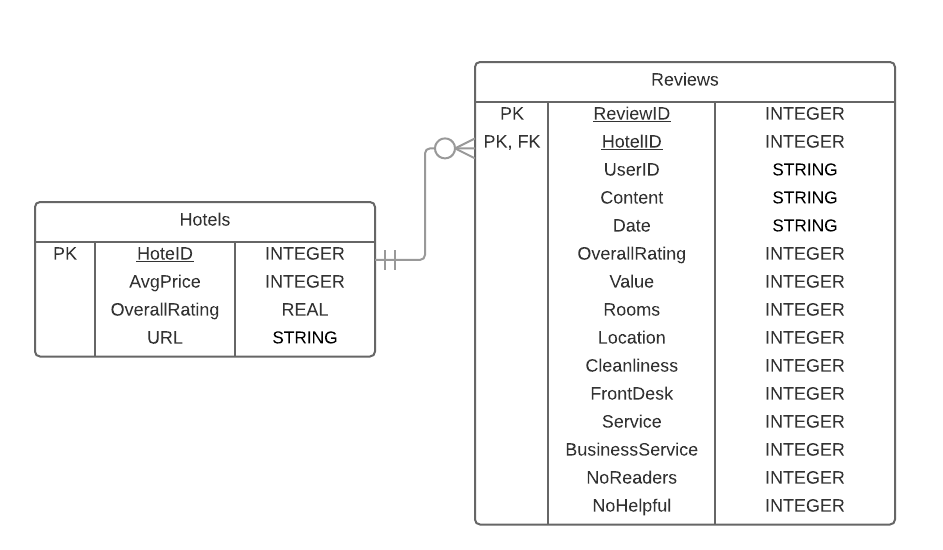
\includegraphics[scale=0.6]{ERD_DIAGRAM.png} 

\section{Relational Algebra}

\subsection{Table Creation}

Finds all reviews by the same user, where x = UserID.
\begin{equation}
	R = \sigma_{username\ \equiv\ x}(Reviews)
\end{equation}

Finds UserID and number of reviews by users with more than 2 reviews.
\begin{equation}
	R =\pi_{UserID,  noReviews}(\gamma_{UserID,COUNT(UserID) \rightarrow noReviews(Reviews)} > 2)
\end{equation}

Finds Hotels with move than 10 reviews.
\begin{equation}
\begin{aligned}
	R = {} & \pi_{HotelID, HotelOverall, HotelAvgPrice, HotelURL} \\
		   & (\gamma_{HotelID,COUNT(HotelID) \rightarrow noReviews(Reviews \bowtie Hotels)} > 10)
\end{aligned}
\end{equation}

Finds Hotels with overall rating greater than 3 and average cleanliness greater than or equal to 5.
\begin{equation}
\begin{aligned}
	R = {} & \{\pi_{HotelID, HotelOverall, HotelAvgPrice, HotelURL}(\sigma_{HotelAvgOverall > 3}(Hotels \bowtie Reviews))\} \\
		   & \cap\ \{\gamma_{HotelID,AVG(Cleanliness) \rightarrow avgMark(Hotels \bowtie Reviews)} \geq 5\}
\end{aligned}
\end{equation}

\section{SQL Queries}

The main table in to which values are read:
\begin{verbatim}
	CREATE TABLE HotelReviews 
	(
		REVIEWID INT NOT NULL,
		HOTELID INT NOT NULL,
		USERID TEXT NOT NULL,
		CONTENT TEXT,
		DATE TEXT NOT NULL,
		OVERALL_RATING INT NOT NULL,
		VALUE INT,
		ROOMS INT,
		LOCATION INT,
		CLEANLINESS INT,
		CHECKIN_FRONTDESK INT,
		SERVICE INT,
		BUSINESS_SERVICE INT,
		NO_READERS INT,
		NO_HELPFUL INT,
		HOTEL_OVERALL REAL NOT NULL,
		HOTEL_AVG_PRICE INT NOT NULL,
		HOTEL_URL TEXT,
		PRIMARY KEY (REVIEWID, HOTELID)		
	);
\end{verbatim}
\paragraph{}
The normalised versions of the tables:
\begin{verbatim}
	CREATE TABLE Reviews 
	(
		REVIEWID INT NOT NULL,
		HOTELID INT NOT NULL,
		USERID TEXT NOT NULL,
		CONTENT TEXT,
		DATE TEXT NOT NULL,
		OVERALL_RATING INT NOT NULL,
		VALUE INT,
		ROOMS INT,
		LOCATION INT,
		CLEANLINESS INT,
		CHECKIN_FRONTDESK INT,
		SERVICE INT,
		BUSINESS_SERVICE INT,
		NO_READERS INT,
		NO_HELPFUL INT,
		PRIMARY KEY (REVIEWID, HOTELID)		
	);
\end{verbatim}
\begin{verbatim}
	CREATE TABLE Hotels
	(
		HOTELID INT PRIMARY KEY NOT NULL,
		HOTEL_OVERALL REAL NOT NULL,
		HOTEL_AVG_PRICE INT NOT NULL,
		HOTEL_URL TEXT
	);
\end{verbatim}

To copy the data into the normalised tables I used the following SQL commands:
\begin{verbatim}
	INSERT INTO Reviews (REVIEWID, HOTELID, USERID ,CONTENT, DATE, OVERALL_RATING, VALUE, ROOMS, LOCATION, CLEANLINESS, CHECKIN_FRONTDESK, SERVICE,	BUSINESS_SERVICE, NO_READERS, NO_HELPFUL)
	SELECT REVIEWID, HOTELID, USERID ,CONTENT, DATE, OVERALL_RATING, VALUE, ROOMS, LOCATION, CLEANLINESS, CHECKIN_FRONTDESK, SERVICE, BUSINESS_SERVICE, NO_READERS, NO_HELPFUL
	FROM HotelReviews;
\end{verbatim}
Above Only the required fields are selected.
\begin{verbatim}
	INSERT INTO Hotels (HOTELID, HOTEL_OVERALL, HOTEL_AVG_PRICE, HOTEL_URL)
	SELECT HOTELID, HOTEL_OVERALL, HOTEL_AVG_PRICE, HOTEL_URL
	FROM HotelReviews
	GROUP BY HOTELID;
\end{verbatim}
In this statement the reviews were grouped by hotel as we only need the attributes related to the hotel, not the review, and each hotel must only appear once as it is the primary key.

Useful indexes would be HotelID and ReviewID in the Reviews table as these are the primary keys, and a HotelID index in the Hotels table where it is also a primary key. One may also wish to index by UserID in the reviews table, as you may wish to aggregate information about users such as how many reviews they have. A HotelOverall index could be useful in order to quickly compare Groups of Hotels with a certain overall rating. An example of an index creation statement would be:

\begin{verbatim}
CREATE INDEX OverallRatings
ON Hotels (HOTEL_OVERALL);
\end{verbatim}

\subsection{Data Retrieval and Analysis}
Select rows where userID = "x":
\begin{verbatim}
SELECT * FROM Reviews 
WHERE USERID = 'x';
\end{verbatim}
Select UserID and Number of Reviews where a user has more than 2 reviews:
\begin{verbatim}
SELECT USERID, COUNT(USERID) FROM Reviews 
GROUP BY USERID
HAVING COUNT(USERID) > 2;
\end{verbatim}
Select Hotels with more than 10 reviews:
\begin{verbatim}
SELECT Hotels.* FROM Hotels 
INNER JOIN Reviews 
ON Hotels.HOTELID = Reviews.HOTELID
GROUP BY Reviews.HOTELID
HAVING COUNT(Reviews.HOTELID) > 10;
\end{verbatim}
Select Hotels with overall rating greater than 3 and average cleanliness greater than or equal to 5:
\begin{verbatim}
SELECT * FROM Hotels 
WHERE HOTEL_OVERALL > 3
INTERSECT
SELECT Hotels.* FROM Hotels 
INNER JOIN Reviews 
ON Hotels.HOTELID = Reviews.HOTELID
GROUP BY Reviews.HOTELID
HAVING AVG(Reviews.CLEANLINESS) >= 5;
\end{verbatim}

\begin{appendix}

\end{document}




